\section{Introduction}

The process of conversion of Alternating current into Direct current is known as rectification. For this, Diodes --- which only allow unidirectional flow of current --- are used. Previously, we have constructed a half-wave rectifier, which conducts only during the positive half-cycle of the AC input. To improve on this method, we can allow unidirectional current flow in the output for both the cycles of input signal and rectify it. Such a circuit is called a Full-wave Rectifier.

There are two types of these circuits ---  a center tap full wave rectifier (using two diodes) or a full wave bridge rectifier (using four diodes). In this experiment we will study a full wave bridge rectifier. 

\begin{figure}[H]
    \centering
    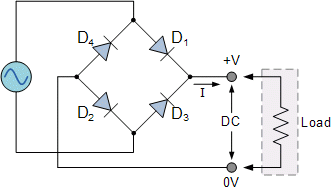
\includegraphics[width=0.7\columnwidth]{images/f1.png}
    \caption{Full-wave rectifier circuit}
    \label{circuit1}
\end{figure}

\section{Theory}

A Full-wave bridge rectifier circuit uses 4 individual rectifying diodes connected in a \textit{bridged} configuration to produce the desired output. The single secondary winding is connected to one side of the diode bridge network and the load to the other side as shown in figure. The 4 diodes labeled D1 to D4 are arranged in "series pairs" with only two diodes conducting current during each half cycle. During the positive half cycle of the supply, diodes D1 and D2 conduct in series while diodes D3 and D4 are reverse biased and the current flows through the load as shown in Fig. 2. During the negative half cycle of the supply, diodes D3 and D4 conduct in series, but diodes D1 and D2 switch of as they are now reverse biased. The current flowing through the load is the same direction as before. 

\begin{figure}[H]
     \centering
     \begin{subfigure}[b]{0.25\textwidth}
         \centering
         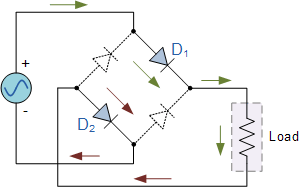
\includegraphics[width=\textwidth]{images/f2.png}
         \caption{}
     \end{subfigure}
     \hfill
     \begin{subfigure}[b]{0.25\textwidth}
         \centering
         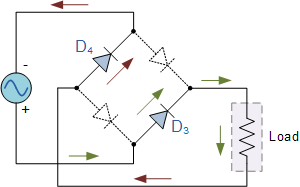
\includegraphics[width=\textwidth]{images/f3.png}
         \caption{}
     \end{subfigure}
     \hfill
        \caption{Working of Full-wave bridge rectifier during (a) positive and (b) negative half cycles}
\end{figure}

We can represent the input AC voltage by 

\begin{equation*}
    V(t) = V_\text{max}\sin(\omega t)   
\end{equation*}

As the current flowing through the load is unidirectional, so the voltage developed across the load is also unidirectional during both the half cycles. Since the signal is repeating itself after every $T/2$ time period, the DC component in the output can be calculated as the time average of $V(t)$ from $0$ to $T/2$, 

\begin{align*}
     V_{\text{dc}} &= \frac{1}{T/2}\int_{0}^{T/2} V(t) \,dt = \frac{2V_{\text{max}}}{\pi} \\
     &=0.637V_{\text{max}}
\end{align*}

Similarly, The RMS of voltage can be calculated using be the time average of $V^2(t)$ from $0$ to $T/2$,

\begin{align*}
    V_{\text{rms}}^2 &= \frac{1}{T/2}\int_{0}^{T/2} V^2(t) \,dt \\
     \implies V_{\text{rms}} &= \frac{V_{\text{max}}}{\sqrt{2}} = 0.707V_{\text{max}}
\end{align*}

\begin{figure}[H]
    \centering
    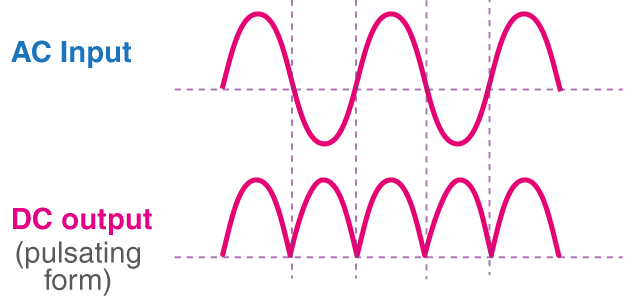
\includegraphics[width=0.65\columnwidth]{images/f0.png}
    \caption{Full-wave rectifier (without filter) input and output waveforms}
\end{figure}

\subsection{Ripple Factor}
The ripple factor is a measure of purity of the d.c. output of a rectifier and is defined as
\begin{equation}
    r = \frac{V_\text{ac}}{V_\text{dc}}
\end{equation}

Where $V_\text{ac}$ and $V_\text{ac}$ are the AC and DC components of the output wavform respectively. Since $V^2_\text{rms} = V^2_\text{ac} + V^2_\text{dc}$,

\begin{align*}
    r &= \sqrt{\frac{V^2_\text{rms} - V^2_\text{dc}}{V^2_\text{dc}}}\\
    &= \sqrt{\frac{V^2_\text{rms}}{V^2_\text{dc}}-1} = \sqrt{\frac{0.707^2}{0.635^2}-1}\\ &= 0.48
\end{align*}

\subsection{Rectification Efficiency}
Rectification efficiency ($\eta$), is a measure of the percentage of total AC power input converted to useful DC power output. 

\begin{align*}
    \eta &= \frac{V_\text{dc}I_\text{dc}}{V_\text{ac}I_\text{ac}}
    = \frac{V^2_\text{dc}/R_L}{V^2_\text{ac}/(r_d+R_L)}\\
    &=\frac{(0.637V_\text{max})^2}{(0.707V_\text{max})^2\left(1+\frac{r_d}{R}\right)} = \frac{0.811}{\left(1+\frac{r_d}{R}\right)}
\end{align*}

where $r_d$ is the forward resistance of the diode. Under ideal conditions ($r_d \approx 0$), the rectification efficiency for a half-wave rectifier is 81.1\%, which is twice the value for a half-wave rectifier.

\subsection{Filters}
The output of a rectifier gives a pulsating DC signal because of presence of some AC components whose frequency is equal to that of the AC supply frequency. To remove any voltage variations or ripples, and smoothen the output, Filter circuits are used. 
In this experiment, we use a smoothing capacitor, which converts the full-wave rippled output of the rectifier into a smooth dc output voltage. 

\paragraph{\textbf{Working Principle}}

\begin{figure}[H]
    \centering
    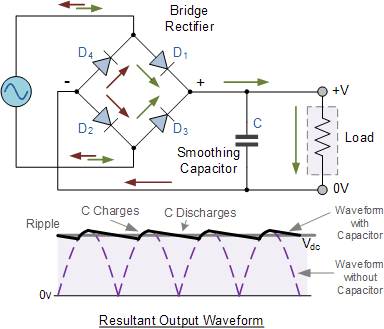
\includegraphics[width=1\columnwidth]{images/f4.png}
    \caption{Full-wave rectifier with a capacitor filter}
    \label{circuit2}
\end{figure}

When the rectifier output voltage is increasing, the capacitor gets charged to its peak voltage $V_m$. Just past that, the rectifier output voltage starts to fall. As the source voltage decreases below $V_m$ , the capacitor will try to send the current back to diode making it reverse biased. Thus the diode separates/disconnects the source from the load and hence the capacitor will discharge through the load until the source voltage becomes more than the capacitor voltage. The diode again starts conducting and the capacitor is again charged to the peak value $V_m$ and the process continues. 

The decay is seen is the exponential decay of any capacitor is charging through a load resistor. The extent to which the capacitor voltage drops depends on the capacitance and the amount of current drawn by the load --- these two factors effectively form the RC time constant for voltage decay. Therefore, two important parameters to consider when choosing a suitable a capacitor are its \textit{working voltage}, which must be higher than the no-load output (with capacitor) value of the rectifier and its \textit{capacitance value}, which determines the amount of ripple that will appear superimposed on top of the dc voltage. 

\subsection{Practical applications}
The main advantages of a full-wave bridge rectifier is that it has a smaller ac ripple value for a given load and requires a smaller smoothing capacitor than an equivalent half-wave rectifier. Improved filters such as a pi-filters can virtually eliminate the amount of ripple voltage that is superimposed on top of the dc supply voltage.

Thus, bridge rectifier circuits are widely used in power supply for various appliances, for powering up the devices which work on DC voltage like motor and led, to detect the amplitude of a modulating radio signal, and so on.